\chapter{Introduction}

\par In this thesis, I discuss the physics of matter in close proximity to neutron stars and black holes.  These astrophysical entities, collectively referred to as `compact objects',  are amongst the most extreme objects in our universe, consisting of several solar masses of matter compressed into an area $\lesssim20$\,km across.  These extreme densities are of interest to material physicists, as understanding matter in this state requires entirely new equations of state.  The environments around these systems have extreme gravitational fields, meaning that these objects are also natural laboratories to test the limits of the theory general relativity \citep{Einstein_GR}.  Neutron stars are also strongly magnetic, piquing the interest of those interested in the dynamics of matter in extreme electromagnetic fields.  As such the study of such objects is of interest to so many physical disciplines, understanding these objects is important to test the limits of our understanding of physics as a whole.
\par Unfortunately, compact objects are inherently faint objects; indeed, an isolated black hole is only visible via the effects its gravitational well has on the light from more distant stars.  As such, observational research into these objects tends to focus one of two types of system: Active Galactic Nuclei (AGNs) and X-Ray Binaries (XRBs).  Both of these systems gravitationally attract matter from their enviroment, a process known as `accretion'.  The energy released by matter falling into such a strong magnetic well causes large amounts of energy to be released; as such, these systems shine brightly in high-energy parts of the electromagnetic spectrum such as the X-rays.
\par AGNs contain supermassive black holes, with masses upwards of $\sim10^6$\,$M_\odot$\footnote{1\,$M_\odot=2\times10^{30}$\,kg, or one times the mass of our Sun.}.  These black holes are present at the centre of almost all large galaxies but many, such as Sagittarius A$^\star$ in our Milky Way, are currently dormant and not significantly accreting.  AGN are the brightest persistent sources of electromagnetic radiation in the universe, and they launch powerful `jets' of matter out to distances of many kpc\footnote{$1$\,kpc$ =1000$\,pc $\approx3\times10^{16}$\,m.}.  AGN have been implicated as having an important role in the development of their host galaxies via a process known as AGN feedback, in which mechanical and electromagnetic power from the AGN are `fed back' into its host galaxy.
\par Active Galactic Nuclei are, almost by definition, very distant systems.  Because of the large distance scales involved, they also only evolve over timescales of thousands of years.  These facts make studying the properties of matter in a relativistic regime by observing AGN somewhat difficult.  Thankfully, there exists a population of bright, accreting compact objects much closer to home: XRBs.

\section{Anatomy of an X-Ray Binary}

\par In this thesis, I will be focusing on XRBs.  These systems are physically much smaller than AGN, with compact objects no more massive than $\sim20\,M_\odot$, but in many ways they can be more extreme.  The gravitational tidal forces close to the compact object are more extreme than in AGN and, due to their small size, XRBs can evolve rapidly over timescales of seconds or less.
\par An XRB is a system containing a compact object and a main sequence or giant companion star.  By various processes, matter is lost from the companion star and transferred onto the compact object.  Due to angular momentum constraints matter cannot simply fall onto the compact object; instead this matter spirals inwards, forming a large disk of material.  Frictional forces in the inner portions this disk heat this disk to extreme temperatures $\gtrsim1$\,keV.  In some XRBs, so much X-ray radiation is released in this process that the pressure from photons becomes important to describe the equation of state of the disk.
\par XRBs are divided into two broad categories depending on the mass of the companion star and, in turn, the predominant mechanism responsible from transferring matter from the star to the compact object.  High Mass X-ray Binaries (HMXBs) have a companion star with a mass $\gtrsim1\,M_\odot$.  Part of the stellar wind from this high-mass companion is gravitationally captured by the compact object, and feeds the accretion disk.
\par Low Mass X-Ray Binaries, systems in which the mass of the companion star is $\lesssim1\,M_\odot$, accrete matter in a different way.  Objects in astrophysical binary systems each have a Roche Lobe: a teardrop-shaped region of space in which that object is gravitationally dominant.  Under some circumstances, it is possible for a star to become larger than its Roche lobe.  This can happen in two ways:
\begin{enumerate}
\item The size of the binary orbit decreases, shrinking the Roche Lobe of each object.
\item The radius of the star increases.  This can happen, for example, when the star evolves from the Main Sequence onto the Giant branch.
\end{enumerate}
In either scenario, a portion of the star ends up within the Roche lobe of the compact object.  This matter is free to spiral onto the compact object, forming the accretion disk.

\subsection{Components of an XRB}

\par In addition to the accretion disk, there are several additional features present in a typical X-Ray Binary; we show a cartoon diagram of an LMXB in Figure \ref{fig:xrbcartoon}.   Radio observations of nearby XRBs have shown that these systems can show axial jets of material similar to those seen in AGN; in Figure \ref{fig:jet} we show a radio image from \citet{Stirling_jet} showing a jet from the HMXB Cyg X-1. xxxxx

\begin{figure}
    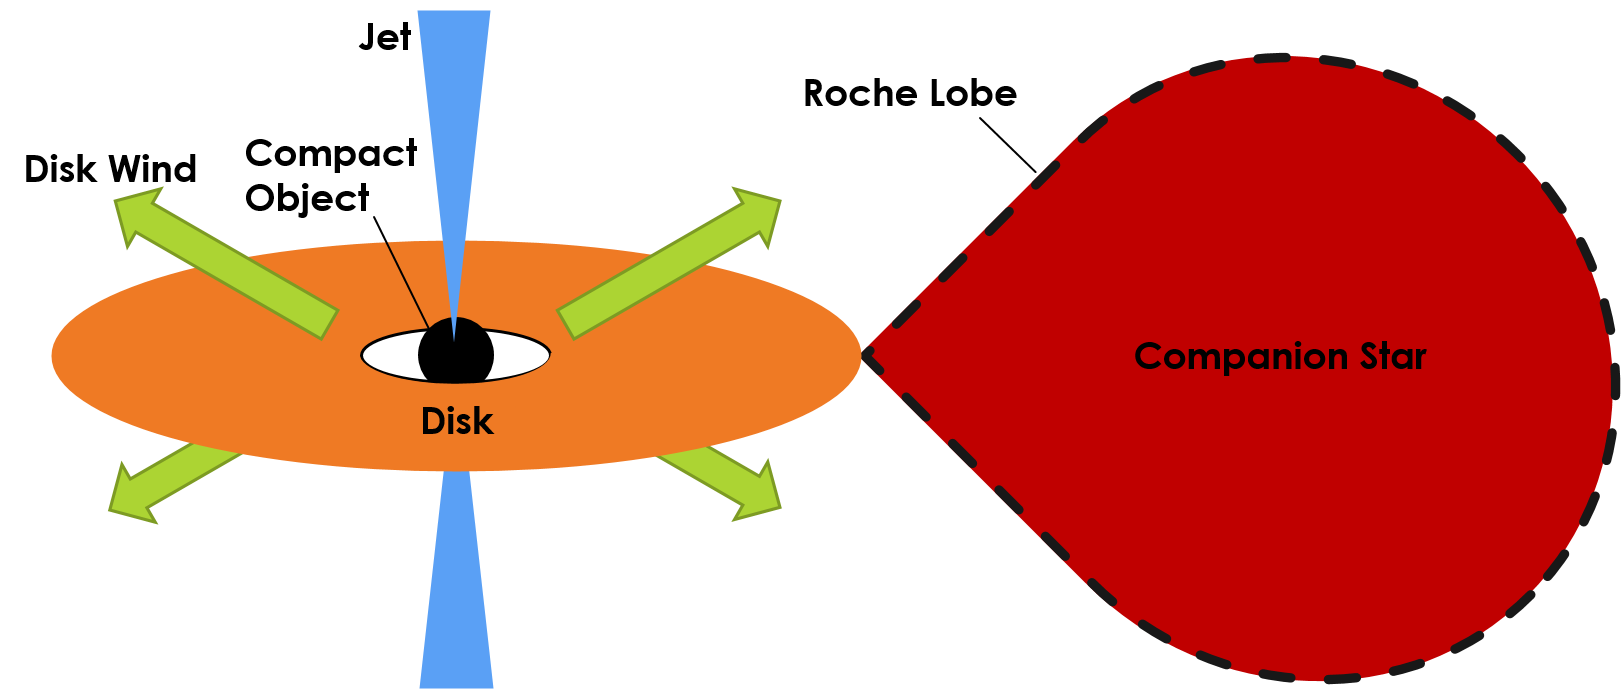
\includegraphics[width=\columnwidth, trim = 0mm 0mm 0mm 0mm]{images/xrbcartoon.eps}
    \captionsetup{singlelinecheck=off}
    \caption{}
   \label{fig:xrbcartoon}
\end{figure}

\begin{figure}
   \centering
    \includegraphics[width=0.6\columnwidth, trim = 17mm 0mm 17mm 0mm, clip]{images/jet.eps}
    \captionsetup{singlelinecheck=off}
    \caption{An 8\,GHz radio image from \citet{Stirling_Jet} showing a jet from the HMX Cyg X-1 (at the origin of the image).  The lowest countour is 0.4\,mJy\,beam$^{-1}$, and other contours represent factors of 2.}
   \label{fig:jet}
\end{figure}

\par X-ray spectral studies of LMXBs find that, in addition to a black-body like accretion disk, the systems must each contain a non-thermal `corona' component.  This corona emits X-rays via Compton upscattering: photons emitted from the disk collide with energetic electrons in the corona.  The photons, on average, gain energy from these collisions and are scattered back into space; some in the direction of observers on the Earth.  This leads to a characteristic energy distribution signature at high energies, which can be seen in the spectra of LMXBs. xxxxx
\par Wind xxxxx



\section{Low Mass X-Ray Binary Behaviour}